%!TEX root = ../main.tex

\section{Accelerated BEM}
\label{sec:fast}

We now focus on a more efficient BEM solver. Indeed, the cost for the solution of standard BEMs remains quadratic: $O(N^2)$, due to the dense structure of their system matrices. This fact poses limitations on the number of degrees of freedom that can be
considered, both in terms of memory requirements and computational times. Exploiting the
structure of the fundamental solution $G$ to approximate the convolution integrals when two
cells are well separated leads to the well-known Fast Multipole Method (FMM), which reduces the computational cost from $O(N^2)$ to $O(N)$. 

\begin{figure*}[!ht]
\begin{center}
    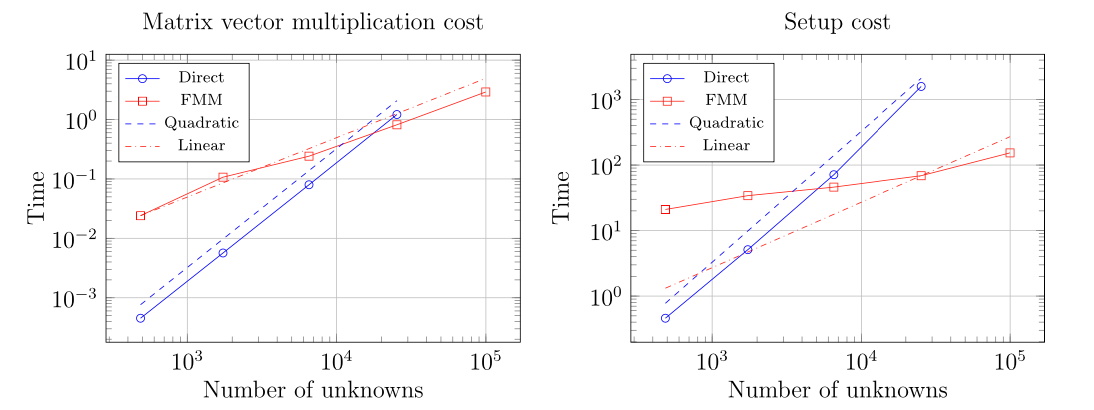
\includegraphics[width=14cm]{original-22}    % The printed column width is 8.4 cm.
    \caption{Computational cost comparison between BEM and BEM-FMM. The figure on the left reports a comparison of a single matrix vector multiplication, the one on the right reports a comparison of the setting time needed by the method.} 
    \label{fig:original-22}
\end{center}
\end{figure*}

\subsection{Fast Multipole Method}
\label{sub:fast_multipole_method}

First, we briefly introduce the FMM. The algorithm was originally derived for $N$-body
problems and it takes into account $N$ evaluation points (nodes) and $M$ charges (sources) that
are distinct in space. $N$-body problems are typical in electromagnetic applications where
one is interested in computing the force exerted by the charges at the evaluation points. The computation is based upon pairwise evaluations of electromagnetic
potential which coincide with the Green functions considered in this paper. This results in the
evaluation of $NM$ source-target distances. If the source and target points coincide, we
recover the quadratic cost $O(N^2)$. The Fast Multipole Method is based on the consideration
that an harmonic expansion of the electromagnetic potential of a single charge allows the
separation into distinct factors of the effects of the source and evaluation point respectively.
In principle, these factors can be computed separately only once for each source and node
point, leading to a $O(N)$ computational cost. In practice, the harmonic series converges only
when target and node points are well separated. Thus, one important building block of the
FMM is a hierarchical space subdivision that is used to decide whether harmonic
expansions or direct potential evaluations are to be used. Observing that the
electromagnetic potential of a single charge coincides with the free space Green functions
employed in most BEM discretisations, it is possible to modify the FMM algorithm and
integrate it into a BEM solver so that we recover the $N$-Body problem. It’s important to
highlight that even if we are considering a complex geometry case and local refinement, we
are still in the FMM framework. This just led to an algorithm that carefully manages the cells in
order to maintain the harmonic convergence, and this is also valid for the weakly singular integrals coming from the boundary integral formulation: we have to deal with specific quadrature formulas, so in such conditions it is not possible to exploit an external FMM library without implementing massive changes while the $\pi$-\texttt{BEM} adapted these characteristics. We
proceed with a comparison between our FMM-BEM and the direct BEM formulation in terms of accuracy and computational costs.

Fig.~\ref{fig:original-22} represents the computational cost comparison between BEM and BEM-FMM. On
the left, it reports a comparison of a single matrix-vector multiplication, and on the right, the setting time needed by the method. As we can see, we obtain the expected linear behavior even if
the break-even point is roughly located at $10^4$ unknowns. For what concerns the accuracy,
the FMM algorithm introduces an error associated with the truncation of the harmonic series
expansions of the type
\begin{equation*}
e_{_\text{FMM}}\leq C \left| \frac{r}{z}  \right|^{p+1}\leq \left( \frac{1}{2}  \right)^{p+1},
\end{equation*}

where $r$ represents the radius of the sphere used to generate the Multipole expansion, $z$ is
the minimum distance between such a sphere and the evaluation node, and $p$ is the truncation order of the Multipole expansion. In FMM algorithm the expansion is only used for sources and nodes lying in \emph{well separated} boxes.

In Fig.~\ref{fig:original-23} we report the convergence rate of the FMM to the direct matrix vector product evaluation (left plot) and to the standard BEM solution (right plot). Also in this case we can see the expected behavior, as the $L_2$ and $L_\infty$ errors lead below the exponential error bounds.

\subsection{FMM Hybrid Parallelisation}
\label{sub:fmm_hybrid_parallelisation}

Here we challenge the parallelisation of FMM-BEM. A key-step is the computation of the so called \emph{Locally Essential Tree} (LET) that drives the overall MPI communication in an optimal way, but one of our implementation choices is the automatic domain decomposition which doesn’t guarantee the construction of such hierarchical tree. This led us to use a multithreaded parallelisation, also due to the
replicated data structures among nodes. We restrict the
distributed memory parallelisation to the most demanding phases of the algorithm by enforcing that the number of threads and the number of MPI processes is kept well balanced at all times. 

Before going on is necessary an overview on the key step of the Fast Multipole Algorithm: in essence, the so-called hierarchical tree is built, which is the name given to the subdivision of the domain into cells that are in turn divided into smaller cells (higher levels).
The last level is represented by the leaves. The algorithm efficiently leverages the multipole expansion at various levels following an ascending phase and a descending phase in which it traverses the levels of the tree. 

\begin{figure*}[!htp]
\begin{center}
    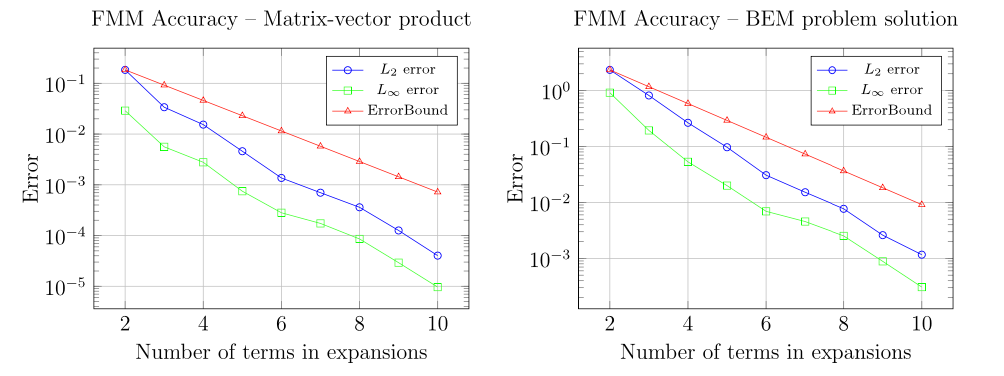
\includegraphics[width=14cm]{original-23}    % The printed column width is 8.4 cm.
    \caption{Convergence analysis for the Multiple expansion using 486 unknowns on the pyramid test case. On the left we report the error of a single matrix vector multiplication, on the right we plot the error on the overall solution.} 
    \label{fig:original-23}
\end{center}
\end{figure*}

One of the most important parameters in the FMM is the number $B$ of evaluation points allowed per leaf of the tree. We want to get some insights on the better tuning of the parameter $B$ to ease the overall computational time of the BEM-FMM algorithm. Greengard and Gropp (see \ref{grop}) derived a simplified analysis of the computational costs to recover an optimal size for the block. We repeat such simplified analysis for the presented FMM in the hybrid shared (TBB) distributed (MPI) memory framework. By defining
\begin{equation*}
\begin{aligned}
N & = \text{number of unknowns}, \\
B & = \text{number of unknowns in a leaf}, \\
p & = \text{number of MPI processors}, \\
t & = \text{number of TBB threads}, 
\end{aligned}
\end{equation*}
the FMM can be sketched as:
\begin{equation}
\label{eq:sum-TFMM}
T_{\text{FMM}} = T_{\text{ascending}} + T_{\text{descending}} + T_{\text{direct}} + T_{\text{comm}},
\end{equation}

where $T_{\text{ascending}}$ represents the time needed by the ascending phase, $T_{\text{descending}}$ is the time needed by the descending phase, $T_{\text{direct}}$ represents the time needed by the short range interactions, while $T_{\text{comm}}$ is the time required by the parallel communications or
synchronisations. If we expand all the terms in Eq.~\eqref{eq:sum-TFMM} we obtain
\begin{equation}
\label{eq:complex-T-formula}
\begin{aligned}
T_{\text{FMM}} =& K_1 \frac{N}{t}+K_2\log_8\left( \frac{N}{B}  \right)\frac{N}{Bt}+K_3\log_8  \left( \frac{N}{B}  \right)\frac{N}{Btp} \\
& +K_4\frac{N}{tp}+K_5\frac{NB}{tp} + e(B,p,t),
\end{aligned}
\end{equation}

where $K_1, K_2, K_3, K_4, K_5$ are experimentally constants that depend on the characteristic of the underlying computational architecture considered, and the function $e$ represents the communication and synchronization cost. Eventually, it can be
easily recover the optimal $B$ by computing the partial derivative of $T_{\text{FMM}}$ with respect to $B$:
\begin{equation}
B_{\text{opt}}=\sqrt{\frac{(K_2+K_3/p)\log_8(N)}{K_5/p} }.
\end{equation}

Fig.~\ref{fig:original-24} represents analysis of the time needed by the overall FMM, considering 1 MPI processor and up to 10 threads per processor, with the number of evaluation nodes per block $B$ varying from 20 to 140. In blue are reported theoretical results using Eq.~\eqref{eq:complex-T-formula}, in green we can see the experimental results. That drastic loss of performance we see is due to the cache-misses. The result is promising since we get that $B_{\text{opt}}=52.5440911254$.

\begin{figure}[!htp]
\begin{center}
    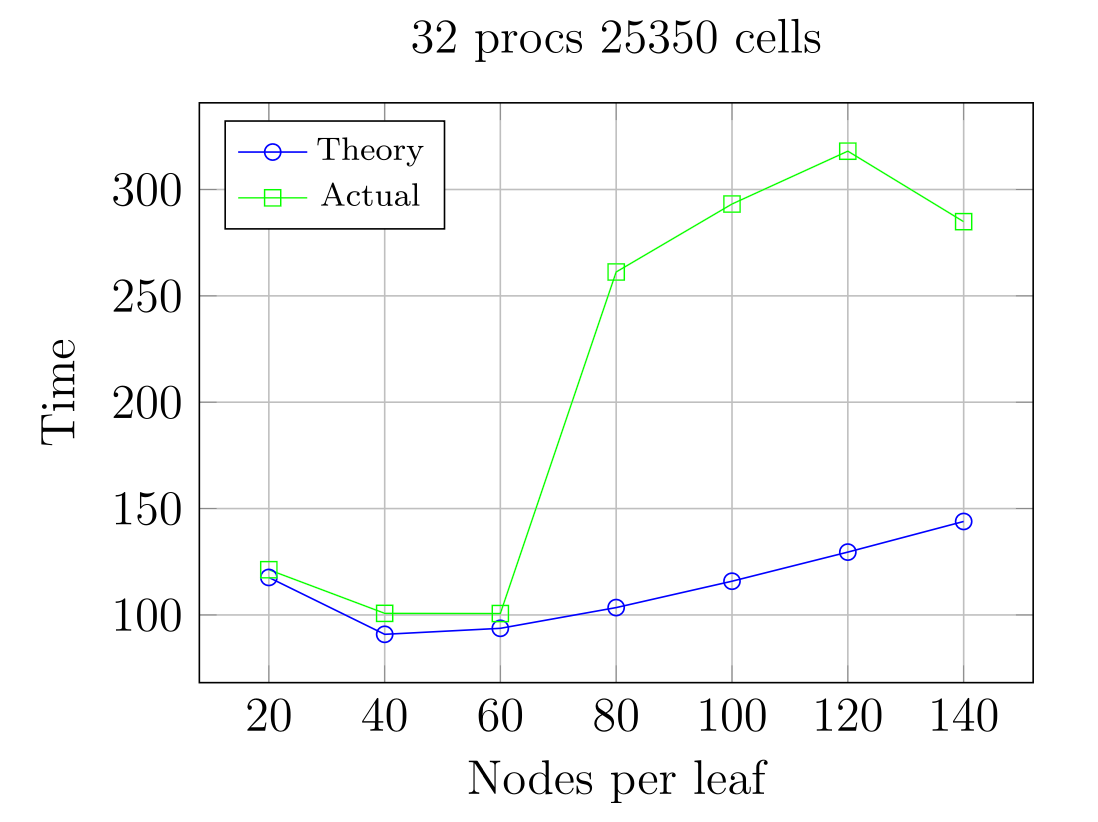
\includegraphics[width=8cm]{original-24}    % The printed column width is 8.4 cm.
    \caption{Analysis of the time needed by the overall FMM.} 
    \label{fig:original-24}
\end{center}
\end{figure}

So for the further analysis we are considering $B$ equal to 60. We highlight that $B_{\text{opt}}$ depends on the number of MPI processor. However, since our FMM is mostly shared memory parallelised, we are not interested in requiring many MPI processors, thus $B = 60$ is a good choice for the scaling analysis.

\subsection{FMM Scaling}
\label{sub:fmm_scaling}

\begin{figure}[!htp]
\begin{center}
    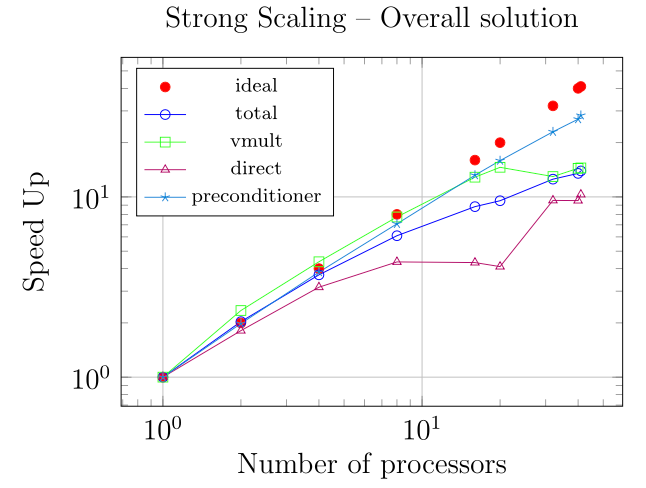
\includegraphics[width=7cm]{original-25-1} \\
    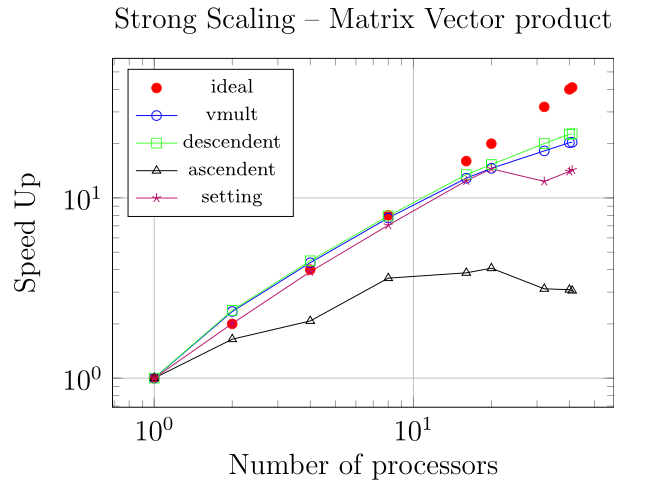
\includegraphics[width=7cm]{original-25-2} % The printed column width is 8.4 cm.
    \caption{Strong Scalability test using 98306 degrees of freedom.} 
    \label{fig:original-25}
\end{center}
\end{figure}

The strong scaling of BEM-FMM algorithm is run
with hybrid TBB-MPI parallelisation up to 2 nodes, each node is composed by two 10 cores, as the previous ones. The top of Fig.~\ref{fig:original-25} represents the strong scaling analysis of the overall algorithm while the bottom illustrates the scalability concerning a single matrix vector multiplication. These plots highlight the scalability issue for short range interactions, and the matrix vector products. Part of the performance loss is induced by the augmented number of iterations needed by the iterative solver when MPI is involved, as suggested by the bottom plot. That plot shows how our
preconditioner is not optimal with rispect to the number of MPI processes. We highlight how the trade-off between computational efficiency and memory is still being studied for a better implementation of the FMM-BEM algorithm, even though we believe the main improvement should come from a better preconditioner.








